\chapter{Event Reconstruction in the CMS detector}
\label{chap:Event}

Events selected by the \ac{CMS} trigger system typically contains signatures of heavy particles, such as the top quark or the Higgs boson. However, the lifetime of these particles are extremely short and they travel a negligible distance before decaying into more stable particles, refer to as the final-state particles. Therefore, the reconstruction of an event produced in the proton-proton collisions requires the identifications of all final state particles, which can be then used to infer the presence of heavy particles. Except for weakly interacting neutrinos, all final-state particles leave traces of their signatures in at least one subsystem of the \ac{CMS} detector as illustrated in Figure~\ref{fig:PF}.

\begin{figure}[tbh!]
 \begin{center}
 \begin{tabular}{c}
 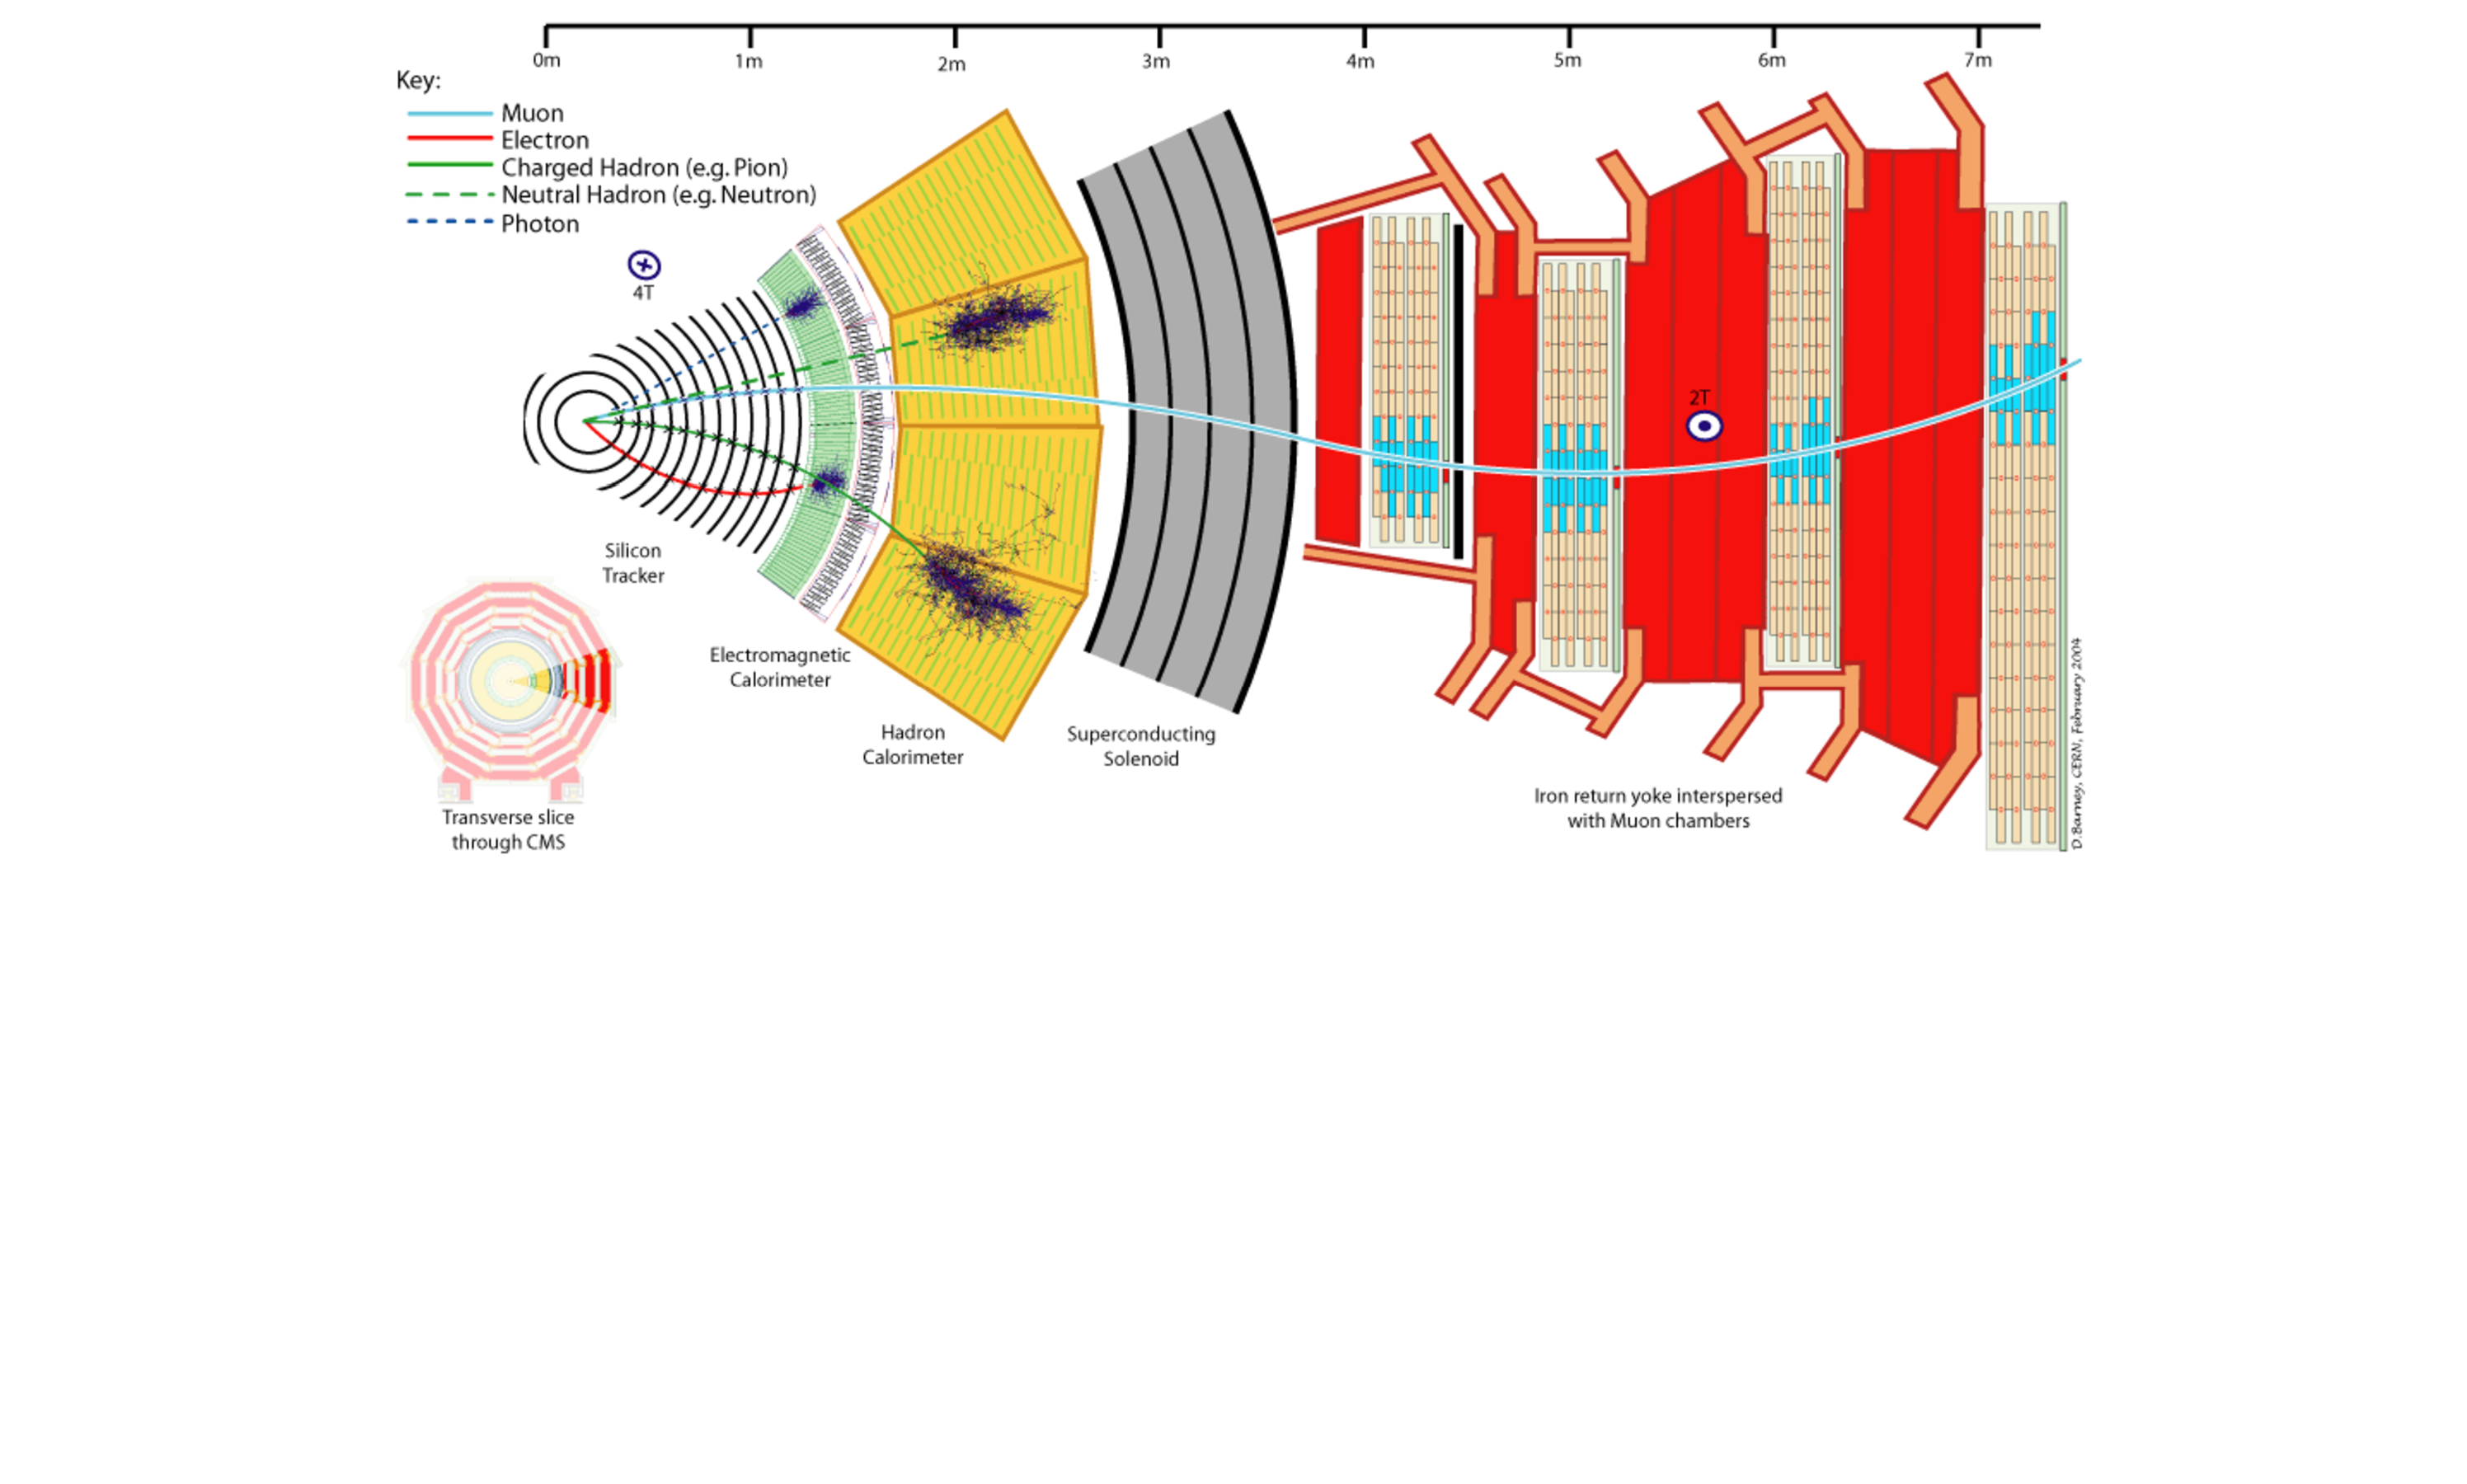
\includegraphics[width=0.9\textwidth]{figures/Part2/Event/PF}
 \end{tabular}
 \caption{A cross-sectional view of a slice of the \ac{CMS} detector in the transverse plane, adapted from~\cite{Barney:2018}. Paths of different particles that interact with various subsystems of the \ac{CMS} detector are highlighted.}
 \label{fig:PF}
 \end{center}
\end{figure}

The \ac{PF} algorithm~\cite{CMS:2017yfk} is used by the \ac{CMS} to combine measurements from all subsystems and provide a global event description. This algorithm consists of two main steps: i) reconstructing the \ac{PF} elements (i.e. tracks and calorimeter clusters) using information from various subsystems and ii) linking these \ac{PF} elements together to form the \ac{PF} objects. The \ac{PF} objects include electrons, photons, muons, charged hadrons, and neutral hadrons. Descriptions of the track and vertex reconstruction are given in \autoref{sec:Track}. The reconstruction of \ac{PF} electrons and muons are discussed in \autoref{sec:Electron} and \autoref{sec:Muon}, respectively. The \ac{PF} objects are also used to reconstruct hadronic jets, taus and \ac{MET}, which is discussed in \autoref{sec:Jet}, \autoref{sec:Tau}, and \autoref{sec:MET}, respectively.

\section{Track and Vertex}
\label{sec:Track}

Tracks from the inner tracking system and the muon system serve as the one of the basic elements of the \ac{PF} algorithm. The standard track reconstruction algorithm at \ac{CMS} is the so called Combinatorial Track Finder (CTF)~\cite{Speer:2005dp}, which is an extension of the the \ac{KF} algorithm~\cite{Fruhwirth:1987fm} that combines the pattern recognition and parameter fitting. The procedure starts by forming a seed using only two or three hits. Initial estimate of the track parameters and their uncertainties are also made in the seeding stage. A \ac{KF}-based pattern recognition is then used to build track candidates by propagating the trajectory of each seed to its nearby surfaces. If a hit is found in the expected window it is added to the candidate track while the track parameter is updated at the same time. The improved knowledge of the track parameter as a result of newly added hits allows for a tighter window for the next propagation. The update of the track parameter is done using a \ac{KF} that performs an iterative fit to track parameters as new hits are added. Lastly, a set of track quality selection criteria is applied to reduce the number of tracks that can not be associated to any particles, known as fake tracks. 

Reconstructed tracks can also be linked together to form a vertex. Vertices that are associated to inelastic scatterings of a collision event is known as the \ac{PV}. Due to the presence of \ac{PU}, multiple \acp{PV} exist in any given collision event. Three main steps are involved in the reconstruction of the \acp{PV}. Firstly, a set of selection criteria is applied to reconstructed tracks to ensure they are are promptly produced in the collisions. Secondly, reconstructed tracks are clustered into a vertex candidate based on their $z$-coordinates using the deterministic annealing algorithm~\cite{Rose:1998dzq}. Finally, candidate vertices with more than one associated track are fitted using adaptive vertex fitter~\cite{Fruhwirth:2007hz}. For each event, the \ac{PV} with highest $\sum\pt^2$ is often considered to be of the most importance to particle physicists as they carry the largest momentum transfer in an event. It is sometimes referred to as simply the \ac{PV} of an event while other \acp{PV} are considered to originate from \ac{PU}.

\section{Electron}
\label{sec:Electron}

Charged particles may emit photons in a process called the \emph{bremsstrahlung}. The intensity of this effect is inversely proportional to the squared mass of the charged particles. As the lightest charged particles, electrons produced in the hadron collisions are heavily affected by the bremsstrahlung effect, which comes in two different aspects. Firstly, the emission of a photon alters the electron trajectory, which undermines the performance of the standard tracking algorithm. A dedicated algorithm known as the Gaussian sum filter~\cite{Adam_2005} is therefore used to fit the electron parameters. Moreover, the bremsstrahlung photons emitted by electrons often cause a more widespread pattern of \ac{ECAL} clusters along the $\phi$ direction. Therefore, multiple adjacent \ac{ECAL} clusters are combined to form the so called \emph{superclusters}.

The electron reconstruction is fully integrated into the \ac{PF} framework, which associates GSF tracks from the inner tracking system to the \ac{ECAL} clusters. The final assignment of the electron energy is based on a weighted combination of the \ac{ECAL} super cluster energy and tracker momentum~\cite{Baffioni:2006cd}. In addition to the electron reconstruction, identification criteria are often applied and optimized for different analyses. For both analyses described in this thesis, the primary objective of the electron identification is to control the contamination of the \emph{nonprompt} leptons. To this end, a \ac{BDT}-based electron identification is deployed, which is discussed in \autoref{sec:Leptons}.

\section{Muon}
\label{sec:Muon}

Three types of muon tracks exist: standalone muons, tracker muons, and global muons~\cite{CMS:2018rym}. The standalone muons refer to the muon tracks reconstructed purely from hits in the muon system. The tracker muons are built ``inside-out'' by propagating tracks from the tracker to the muon system and match it with and at least one hit from the \ac{CSC} or \ac{DT}. The global muon is reconstructed ``outside-in'' by: i) matching the standalone muons with the inner tracks and ii) performing a combined fit using the \ac{KF} to update the muon parameters. 

Same as the electron, the muon reconstruction is fully integrated into the \ac{PF} algorithm, which applies a set of selection criteria based on quality parameters in the muon reconstruction to all three types of muon tracks. The so called Medium muon ID~\cite{CMS:2018rym} is used by by analyses described in this thesis. This ID accepts both tracker muons and global muons and adjusts the selection criteria accordingly. The overall efficiency of this ID is estimated to be around 99.5\%  for muons from simulated W and Z events.

\section{Jet}
\label{sec:Jet}

This chapter summarizes the offline reconstruction techniques used by the \ac{CMS} in order to identify the final-state particles. Descriptions of the track and vertex reconstruction are given in \autoref{sec:Track}. \autoref{sec:Electron} and \autoref{sec:Muon} discuss the reconstruction of electrons and muons, respectively. \autoref{sec:Tau} and \autoref{sec:Jet} discuss the reconstruction of hadronic jets and taus, respectively. The reconstruction of the \ac{MET} is discussed in \autoref{sec:MET}.

\section{Hadronic Tau}
\label{sec:Tau}

This chapter summarizes the offline reconstruction techniques used by the \ac{CMS} in order to identify the final-state particles. Descriptions of the track and vertex reconstruction are given in \autoref{sec:Track}. \autoref{sec:Electron} and \autoref{sec:Muon} discuss the reconstruction of electrons and muons, respectively. \autoref{sec:Tau} and \autoref{sec:Jet} discuss the reconstruction of hadronic jets and taus, respectively. The reconstruction of the \ac{MET} is discussed in \autoref{sec:MET}.

\section{Missing Transverse Momentum}
\label{sec:MET}

This chapter summarizes the offline reconstruction techniques used by the \ac{CMS} in order to identify the final-state particles. Descriptions of the track and vertex reconstruction are given in \autoref{sec:Track}. \autoref{sec:Electron} and \autoref{sec:Muon} discuss the reconstruction of electrons and muons, respectively. \autoref{sec:Tau} and \autoref{sec:Jet} discuss the reconstruction of hadronic jets and taus, respectively. The reconstruction of the \ac{MET} is discussed in \autoref{sec:MET}.